\section{Adding Lattices to Bloom}
\label{sec:impl}

\begin{figure}[t]
\begin{scriptsize}
\begin{lstlisting}
class ShortestPaths
  include Bud

  state do
    table :link, [:from, :to, :c]
    table :path, [:from, :to, :next_hop] => [:c]
    table :min_cost, [:from, :to] => [:c]
  end

  bloom do
    path <= link {|l| [l.from, l.to, l.to, MinLattice.new(l.c)]}
    path <= (link*path).pairs(:to => :from) do |l,p|
      [l.from, p.to, l.to, p.c + l.c]
    end
    min_cost <= path {|p| [p.from, p.to, p.c]}
  end
end
\end{lstlisting}
\end{scriptsize}
\caption{A \lang program to compute the all-pairs shortest paths of a
  graph.}
\label{fig:lattice-spaths}
\end{figure}

% Outline:
% * design philosophy, sign posting
% * introduce lattice values
% * introduce lattice wrappers
% * introduce morphisms
% * discuss example program
% * discuss integration features
% * implementation notes

% XXX: need intro paragraph

% is this the right place for this?
When designing \lang, we decided to extend Bloom to include support for
lattices rather than building a new language from scratch. Hence, \lang is
backward compatible with Bloom, and was implemented with relatively minor
changes to the Bud runtime. This design decision also required that we consider
rules written over lattices should interoperate with rules that use traditional
Bloom relations; we added several \lang features to ease this interoperability,
which we describe in Section~\ref{sec:bloom-interop}.

\subsection{Lattice classes and elements}
In \lang, each lattice has an associated Ruby class, which we call the
\emph{lattice class}. An instance of this class is called a \emph{lattice
  element}. A lattice element represents a single point in the lattice---i.e., an
element of the poset associated with the lattice.

A lattice class is a normal Ruby class that meets a certain API contract. Every
lattice class inherit from the builtin \texttt{Bud::Lattice} class, and
must also define two methods:
\begin{itemize}
\item \texttt{initialize(i)}: given a Ruby object \emph{i}, this method
  constructs a new lattice element that ``wraps'' \emph{i} (\texttt{initialize}
  is just the normal Ruby syntax for defining a constructor). By convention, the
  Ruby value wrapped by a lattice element is assigned to a Ruby member variable
  \texttt{@v}. If $i$ is the null reference, this method returns the least
  element of the lattice.

\item \texttt{merge(e)}: given a lattice element \emph{e}, this method returns the
  lattice element that is the least upper bound of $\{e, \textit{self}\}$. This method must
  satisfy the algebraic properties summarized in Section~\ref{sec:found-defn}---in
  particular, it must be commutative, associative, and idempotent. Note that
  \emph{e} must have the same class as \emph{self}.
\end{itemize}
Lattice elements are \emph{immutable} (e.g., \texttt{merge} functions should
construct a new lattice element rather than modifying one of their inputs
in-place). Efficient lattice implementations may \emph{share structure} on merge
operations, as is common practice for immutable data structures in functional
programming languages~\cite{Okasaki1999}. % XXX: maybe not the right place for this

\subsection{Morphisms and OPMs}
As described in Section~\ref{sec:foundation}, morphisms allow complex programs
to be created via the composition of multiple lattices. In \lang, a morphism is
akin to a Ruby method that satisfies the algebraic properties summarized in
Section~\ref{sec:found-defn}.

\subsection{Program analysis}

\begin{figure}[t]
\begin{scriptsize}
\begin{lstlisting}
class Bud::SetLattice < Bud::Lattice
  wrapper_name :lset

  def initialize(x=[])
    @v = x     # Reject invalid input (elided)
  end

  def merge(i)
    self.class.new(@v | i.reveal)
  end

  morph :intersect do |i|
    self.class.new(@v & i.reveal)
  end

  morph :pro do |&blk|
    @v.map(&blk)
  end

  ord_map :size do
    Bud::MaxLattice.new(@v.size)
  end
end
\end{lstlisting}
\end{scriptsize}
\caption{The implementation of the \texttt{lset} lattice in Ruby.}
\label{fig:lattice-set}
\end{figure}

\subsection{Integration with set-oriented logic}
\label{sec:bloom-interop}

\lang provides two features to ease integration of lattice-based code with
traditional Bloom programs that manipulate set-oriented collections.

\subsubsection{Implicit fold}
% XXX: this ignores the fact that Bloom collections consist of sets of tuples,
% whereas implicit fold works for sets of singleton values
% XXX: refer to shortest paths program as practical example
This feature enables set-oriented collections to be more easily used as input to
lattices. If a \lang rule has a set-oriented collection on the rhs and a lattice
on the lhs, the lattice merge function is used to ``fold over'' the elements of
the collection. That is, each element of the collection is converted to a
lattice element (via the appropriate lattice constructor); then the set of
lattice elements are merged together (via repeated application of the
\texttt{merge} method). In our experience, this is typically the behavior
intended by the user.

\subsubsection{Collections with embedded lattice values}
It would be convenient to allow lattice elements to be stored as attributes of
tuples that appear in set-oriented Bloom collections. Furthermore, Bloom
provides several facilities (e.g., network communication, persistent storage,
module interfaces) as collections with special semantics; it would be
unfortunate if a redundant set of facilities would be necessary to support
lattice-based code. Naturally, lattice-based \lang code could interact with
set-oriented collections by extracting the underlying Ruby value from the
lattice (e.g., using the \texttt{reveal} method), but this would needlessly
introduce non-monotonicity into the program.

Storing lattice elements as attributes of tuples in set-oriented collections
introduces several challenges. Tuples in Bloom collections are traditionally
immutable: once a fact is known to be true, its value remains the
same.\footnote{Bloom facts can be explicitly deleted, but this is a
  non-monotonic operation that can only occur between timesteps. Conceptually,
  Bloom models update as the retraction of the previous version of a fact and
  the insertion of a new fact~\cite{dedalus}.}

\subsection{Implementation}

\subsubsection{Lattice wrappers}
A \emph{lattice wrapper} manages the mapping from identifier names to lattice
elements.

\begin{table*}[t]
\begin{tabular}{|l|l|l|l|l|}
\hline
\textbf{Name} & \textbf{Description} & \textbf{Merge} & \textbf{Morphisms} & \textbf{OPMs}\\
\hline
\texttt{lbool} & Boolean lattice (false $\to$ true) & & \texttt{when\_true} & \\
\texttt{lmax} & Max over an ordered domain & &\texttt{gt},
\texttt{gt\_eq}, \texttt{+}, \texttt{-} & \\
\texttt{lmin} & Min over an ordered domain & &\texttt{lt}, \texttt{lt\_eq},
\texttt{+}, \texttt{-} & \\
\texttt{lset} & Set of values & & \texttt{intersect}, \texttt{product},
\texttt{project} & \texttt{size} \\
\texttt{lpset} & Set of non-negative numbers & &
\texttt{intersect}, \texttt{project}& \texttt{size}, \texttt{sum} \\
\texttt{lbag} & Multiset of values & & \texttt{intersect},
\texttt{project}, \texttt{mult(k)} & \texttt{size}\\
\texttt{lmap} & Map from key to lattice values & &
\texttt{intersect}, \texttt{project}, \texttt{at(k)}, \texttt{key?(k)} & \texttt{size}\\
\hline
\end{tabular}
\caption{The builtin lattice types in \lang.}
\label{tbl:builtin-lattices}
\end{table*}

\subsection{Performance study}

\begin{figure}
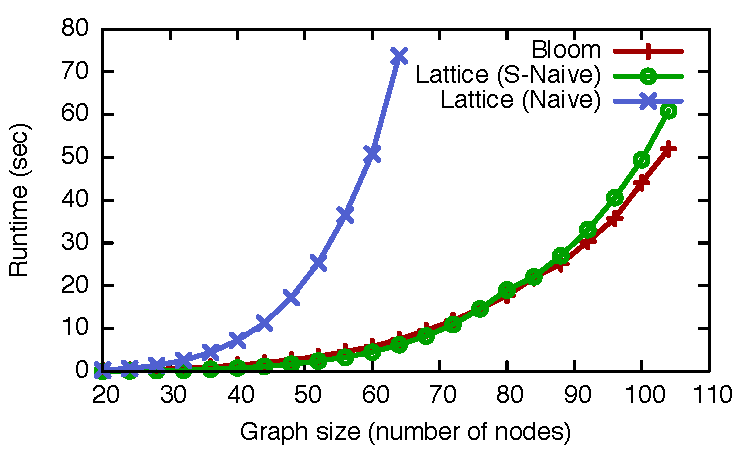
\includegraphics[width=\linewidth]{fig/sn_perf}
\caption{Performance comparison of several different transitive closure
  programs.}
\label{fig:tc-perf-graph}
\end{figure}